\aula{04b}{10}{setembro}{2026}

\begin{resposta}
    \begin{enumerate}[start=9]

        \item Dimensionamento armaduras negativas
        
        \begin{figure}[H]
    \centering
    \begin{tikzpicture}[
        scale=1.5,
        retangulo/.style={draw=gray!80!black, thick},
        rotuloLetra/.style={font=\footnotesize, blue!80!black},
        eixo/.style={->, >=stealth, thick, black},
        corte/.style={draw=black, dash dot, thick},
        setaCorte/.style={->, >=stealth, thick, black}
    ]

        % --- Definição dos Parâmetros de Dimensão ---
        \def\wCentro{3.2}       % Largura dos retângulos centrais (L1 e L3)
        \def\hCima{2.0}         % Altura do retângulo superior (L1)
        \def\hBaixo{2.2}        % Altura do retângulo inferior (L3)
        
        \def\wDir{2.2}          % Largura do retângulo da direita (L2)
        \def\hDir{\hCima + \hBaixo} % Altura total da laje L2
        
        \def\wEsq{1.6}          % Largura do retângulo da esquerda (L4)
        \def\hEsq{\hBaixo}      % Altura da laje L4

        % --- Coordenadas ---
        \coordinate (A2) at (0, 0);
        \coordinate (B2) at (\wCentro, 0);
        \coordinate (C2) at (\wCentro, \hBaixo);
        \coordinate (D2) at (0, \hBaixo);

        \coordinate (A1) at (0, \hBaixo);
        \coordinate (B1) at (\wCentro, \hBaixo);
        \coordinate (C1) at (\wCentro, \hBaixo + \hCima);
        \coordinate (D1) at (0, \hBaixo + \hCima);

        \coordinate (A3) at (\wCentro, 0);
        \coordinate (B3) at (\wCentro + \wDir, 0);
        \coordinate (C3) at (\wCentro + \wDir, \hDir);
        \coordinate (D3) at (\wCentro, \hDir);

        \coordinate (A4) at (-\wEsq, 0);
        \coordinate (B4) at (0, 0);
        \coordinate (C4) at (0, \hEsq);
        \coordinate (D4) at (-\wEsq, \hEsq);

        % --- Desenho dos Retângulos ---
        \draw[retangulo] (A1) rectangle (C1); % L1
        \draw[retangulo] (A2) rectangle (C2); % L3
        \draw[retangulo] (A3) rectangle (C3); % L2
        \draw[retangulo] (A4) rectangle (C4); % L4

        % --- EIXOS LOCALIZADOS COM NÚMERO NO CENTRO DE CADA EIXO ---
        % L1 (Topo)
        \coordinate (CL1) at ($(A1)!0.4!(C1)$);
        \draw[eixo] (CL1) -- ($(CL1)+(0.55,0)$) 
            node[midway, below=2pt, blue!80!black, fill=white, inner sep=1pt, font=\footnotesize] {0,76} 
            node[right=-2pt, font=\small] {$y$};
        \draw[eixo] (CL1) -- ($(CL1)+(0,0.55)$) 
            node[midway, left=2pt, blue!80!black, fill=white, inner sep=1pt, font=\footnotesize] {2,43} 
            node[above=-2pt, font=\small] {$x$};

        % L3 (Baixo)
        \coordinate (CL3) at ($(A2)!0.4!(C2)$);
        \draw[eixo] (CL3) -- ($(CL3)+(0.55,0)$) 
            node[midway, below=2pt, blue!80!black, fill=white, inner sep=1pt, font=\footnotesize] {5,36} 
            node[right=-2pt, font=\small] {$x$};
        \draw[eixo] (CL3) -- ($(CL3)+(0,0.55)$) 
            node[midway, left=2pt, blue!80!black, fill=white, inner sep=1pt, font=\footnotesize] {4,04} 
            node[above=-2pt, font=\small] {$y$};

        % L4 (Esquerda)
        \coordinate (CL4) at ($(A4)!0.4!(C4)$);
        \draw[eixo] (CL4) -- ($(CL4)+(0.55,0)$) 
            node[midway, below=2pt, blue!80!black, fill=white, inner sep=1pt, font=\footnotesize] {-1,10} 
            node[right=-2pt, font=\small] {$x$};
        \draw[eixo] (CL4) -- ($(CL4)+(0,0.55)$) 
            node[midway, left=2pt, blue!80!black, fill=white, inner sep=1pt, font=\footnotesize] {0,07} 
            node[above=-2pt, font=\small] {$y$};

        % L2 
        \coordinate (CL2) at ($(A3)!0.5!(C3)$);
        \draw[eixo] (CL2) -- ($(CL2)+(0.55,0)$) 
            node[midway, below=2pt, blue!80!gray, fill=white, inner sep=1pt, font=\footnotesize] {7,80} 
            node[right=-2pt, font=\small] {$x$};
        \draw[eixo] (CL2) -- ($(CL2)+(0,0.55)$) 
            node[midway, left=2pt, blue!80!gray, fill=white, inner sep=1pt, font=\footnotesize] {2,24} 
            node[above=-2pt, font=\small] {$y$};


        % --- LINHAS DE CORTE A, B e C ---
        % Corte A: passa na L1 e L2
        %\draw[corte] (-0.4, 2.85) -- (\wCentro + \wDir + 0.4, 2.85);
        %\draw[setaCorte] (-0.4, 2.85) -- (-0.4, 3.15) node[above, font=\small\bfseries] {A};
        %\draw[setaCorte] (\wCentro + \wDir + 0.4, 2.85) -- (\wCentro + \wDir + 0.4, 3.15) node[above, font=\small\bfseries] {A};

        % Corte B: da L3 a L2 (passando por L4)
        %\draw[corte] (-\wEsq - 0.4, 0.5) -- (\wCentro + \wDir + 0.4, 0.5);
        %\draw[setaCorte] (-\wEsq - 0.4, 0.5) -- (-\wEsq - 0.4, 0.8) node[above, font=\small\bfseries] {B};
        %\draw[setaCorte] (\wCentro + \wDir + 0.4, 0.5) -- (\wCentro + \wDir + 0.4, 0.8) node[above, font=\small\bfseries] {B};

        % Corte C: de L1 a L4
        %\draw[corte] (0.6, \hDir + 0.4) -- (0.6, -0.4);
        %\draw[setaCorte] (0.6, \hDir + 0.4) -- (0.9, \hDir + 0.4) node[right, font=\small\bfseries] {C};
        %\draw[setaCorte] (0.6, -0.4) -- (0.9, -0.4) node[right, font=\small\bfseries] {C};

        % --- Rótulos de Esforço Cortante nas Arestas ---
        % L1 (Topo)
        %\node[below, rotuloLetra] at ($(D1)!0.5!(C1)$) {$V_x$}; 
        %\node[right, rotuloLetra] at ($(D1)!0.5!(A1)$) {$V_y$}; 
        \node[ rotuloLetra, fill=white, inner sep=1pt] at ($(A1)!0.5!(B1)$) {11,54};
        \node[rotuloLetra, fill=white, inner sep=1pt]  at ($(B1)!0.5!(C2)$) {16,04}; 

        % L3 (Baixo)
        %\node[below, rotuloLetra] at ($(A1)!0.5!(B1)$) {$11,54$};
        %\node[right, rotuloLetra] at ($(D2)!0.5!(A2)$) {$0$}; 
        %\node[above, rotuloLetra] at ($(A2)!0.5!(B2)$) {$V_y$};
        %\node[rotuloLetra, fill=white, inner sep=1pt]  at ($(B2)!0.5!(C2)$) {14,77};  
        
        % L2 (Direita)
        %\node[right, rotuloLetra] at ($(B1)!0.5!(C2)$) {$16,04$}; 
        %\node[below, rotuloLetra] at ($(D3)!0.5!(C3)$) {$V_y$}; 
        %\node[left= rotuloLetra]  at ($(C3)!0.5!(B3)$) {$V_x$}; 
        %\node[above, rotuloLetra] at ($(A3)!0.5!(B3)$) {$V_y$}; 

        % L4 (Esquerda)
        \node[rotuloLetra, fill=white, inner sep=1pt]  at ($(D2)!0.5!(A2)$) {13,59}; 
        %\node[below, rotuloLetra] at ($(D4)!0.5!(C4)$) {$V_y$}; 
        %\node[above, rotuloLetra] at ($(A4)!0.5!(B4)$) {$V_y$}; 
        \node[left, rotuloLetra]  at ($(D4)!0.5!(A4)$) {0,98}; 
        \draw[retangulo,white,dashed] (D4) rectangle (A4);
        
        \node[below, right=50pt] at ($(A3)!0.5!(B3)$) {$kN m/m$}; 

    \end{tikzpicture}
    %\caption{Arranjo de lajes com eixos locais numerados e cortes transversais A, B e C}
    %\label{fig:lajes_cortes}
\end{figure}
        
        \fbox{L1-L2} \fbox{L2-L4}

        \begin{figure}[H]
    \centering

    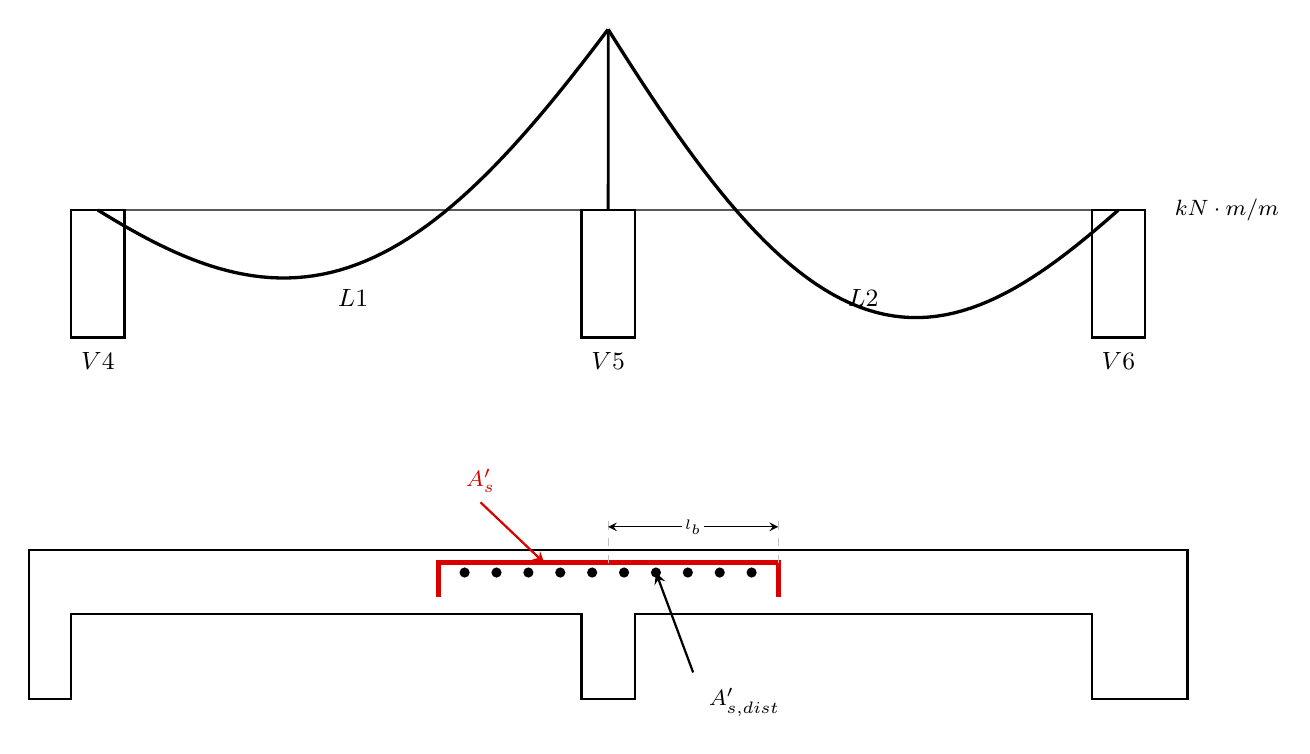
\begin{tikzpicture}[
        scale=1.35,
        pilar/.style={draw=black, thick, fill=white},
        viga/.style={line width=1pt, gray!70!black},
        linhaCompat/.style={line width=1.2pt, black},
        cota/.style={<->, >=stealth, thin, black},
        chamada/.style={gray!50, thin, dashed},
        armaduraNeg/.style={line width=1.8pt, red!85!black},
        armaduraPos/.style={line width=1.5pt, blue!80!black},
        pontoBarra/.style={circle, fill=black, inner sep=1.3pt}
    ]
    
        % --- Parâmetros de Geometria ---
        \def\L{4.8}        % Comprimento de cada vão
        \def\wP{0.5}        % Largura da viga/apoio
        \def\hP{1.2}        % Altura do apoio no diagrama superior
    
        % Coordenadas dos Apoios (V4, V5, V6)
        \coordinate (P1) at (0, 0);
        \coordinate (P2) at (\L, 0);
        \coordinate (P3) at (2*\L, 0);
    
        % ==========================================================
        % 1. DIAGRAMA DE MOMENTOS FLETORES (PARTE SUPERIOR)
        % ==========================================================
        % Eixo das Vigas
        \draw[viga] (0, 0) -- (2*\L, 0);
    
        % Apoios V4, V5, V6
        \draw[pilar] (-\wP/2, -\hP) rectangle (\wP/2, 0);
        \node[below=2pt, font=\small\bfseries] at (0, -\hP) {$V4$};
    
        \draw[pilar] (\L-\wP/2, -\hP) rectangle (\L+\wP/2, 0);
        \node[below=2pt, font=\small\bfseries] at (\L, -\hP) {$V5$};
    
        \draw[pilar] (2*\L-\wP/2, -\hP) rectangle (2*\L+\wP/2, 0);
        \node[below=2pt, font=\small\bfseries] at (2*\L, -\hP) {$V6$};
    
        % Rótulos das Lajes e Unidade
        \node[below=4pt, font=\small\bfseries, fill=white, inner sep=1.5pt] at (\L/2, -\hP/2) {$L1$};
        \node[below=4pt, font=\small\bfseries, fill=white, inner sep=1.5pt] at (1.5*\L, -\hP/2) {$L2$};
        \node[right, font=\footnotesize, fill=white, inner sep=1pt] at (2*\L + 0.5, 0) {$\text{kN}\cdot\text{m/m}$};

        % Conexão vertical do momento no apoio V5
        \coordinate (Pt2) at (\L, 1.7);
        \draw[line width=1pt, black] (\L, 0) -- (Pt2);

        % Curvas de Momento Fletor Compatibilizado
        \draw[linhaCompat] 
            plot[domain=0:\L, samples=60] (\x, {-0.95 * sin(\x * 180 / \L) + 1.7 * (\x/\L)^2});

        \draw[linhaCompat] 
            plot[domain=\L:2*\L, samples=60] (\x, {-1.35 * sin((\x-\L) * 180 / \L) + 1.7 * ((\x-\L)/\L - 1)^2});

        %\node[font=\small\bfseries, align=center] at (\L, 2.3) {Diagrama de Momentos Fletores Compatibilizados};

        % ==========================================================
        % 2. CORTE TRANSVERSAL DA LAJE E DETALHAMENTO DAS ARMADURAS
        % ==========================================================
        \def\yCorte{-3.2}     % Nível do topo da laje no corte
        \def\hLaje{0.6}      % Espessura da laje no desenho
        \def\hVigaCorte{1.4} % Altura total das vigas no corte

        %\node[font=\small\bfseries, align=center] at (\L, \yCorte + 0.95) {Corte Longitudinal da Laje — Detalhamento da Armadura Negativa};

        % Contorno de Concreto (L1 - V5 - L2)
        \draw[thick, fill=white] 
            (-\wP/2 - 0.4, \yCorte) -- (2*\L + \wP/2 + 0.4, \yCorte) --
            (2*\L + \wP/2 + 0.4, \yCorte - \hVigaCorte) -- (2*\L - \wP/2, \yCorte - \hVigaCorte) --
            (2*\L - \wP/2, \yCorte - \hLaje) -- (\L + \wP/2, \yCorte - \hLaje) --
            (\L + \wP/2, \yCorte - \hVigaCorte) -- (\L - \wP/2, \yCorte - \hVigaCorte) --
            (\L - \wP/2, \yCorte - \hLaje) -- (-\wP/2, \yCorte - \hLaje) --
            (-\wP/2, \yCorte - \hVigaCorte) -- (-\wP/2 - 0.4, \yCorte - \hVigaCorte) -- cycle;

        % Rótulos de Vigas e Lajes no Corte
        %\node[font=\small\bfseries] at (0, \yCorte - \hVigaCorte + 0.25) {V4};
        %\node[font=\small\bfseries] at (\L, \yCorte - \hVigaCorte + 0.25) {V5};
        %\node[font=\small\bfseries] at (2*\L, \yCorte - \hVigaCorte + 0.25) {V6};

        %\node[font=\small\bfseries, color=gray!50!black] at (0.35*\L, \yCorte - \hLaje/2) {Laje L1};
        %\node[font=\small\bfseries, color=gray!50!black] at (1.65*\L, \yCorte - \hLaje/2) {Laje L2};

        % --- ARMADURA NEGATIVA PRINCIPAL SOBRE V5 ---
        \def\yArmNeg{\yCorte - 0.12} % Posição superior (abaixo do cobrimento)
        \def\lAncoragem{1.6}         % Comprimento de ancoragem lb
        \def\hGancho{0.32}           % Comprimento do gancho vertical

        % Traçado da Armadura Negativa com Ganchos
        \draw[armaduraNeg] 
            (\L - \lAncoragem, \yArmNeg - \hGancho) -- 
            (\L - \lAncoragem, \yArmNeg) -- 
            (\L + \lAncoragem, \yArmNeg) -- 
            (\L + \lAncoragem, \yArmNeg - \hGancho);

        % --- ARMADURA SECUNDÁRIA (DE DISTRIBUIÇÃO - PONTOS TRANSVERSAIS) ---
        \foreach \xP in {-1.35, -1.05, -0.75, -0.45, -0.15, 0.15, 0.45, 0.75, 1.05, 1.35} {
            \node[pontoBarra] at (\L + \xP, \yArmNeg - 0.09) {};
        }

        % --- ARMADURAS POSITIVAS INFERIORES NAS LAJES L1 E L2 ---
        \def\yArmPos{\yCorte - \hLaje + 0.12}
        %\draw[armaduraPos] (0.1, \yArmPos + \hGancho) -- (0.1, \yArmPos) -- (\L - 0.1, \yArmPos) -- (\L - 0.1, \yArmPos + \hGancho);
        %\draw[armaduraPos] (\L + 0.1, \yArmPos + \hGancho) -- (\L + 0.1, \yArmPos) -- (2*\L - 0.1, \yArmPos) -- (2*\L - 0.1, \yArmPos + \hGancho);

        % --- CHAMADAS E NOTAÇÕES ---
        % 1. Armadura Negativa Principal
        \draw[<-, >=stealth, line width=0.8pt, red!85!black] 
            (\L - 0.6, \yArmNeg) -- (\L - 1.2, \yCorte + 0.45) 
            node[above, font=\footnotesize\bfseries, text=red!85!black] {$A'_s$};

        % 2. Armadura Secundária de Distribuição
        \draw[<-, >=stealth, line width=0.8pt, black] 
            (\L + 0.45, \yArmNeg - 0.09) -- (\L + 0.8, \yCorte - \hLaje - 0.55) 
            node[below right=2pt, font=\footnotesize\bfseries, text=black] {$A'_{s,dist}$};

        % 3. Gancho / Ancoragem
        %\draw[<-, >=stealth, line width=0.8pt, red!85!black] 
            %(\L + \lAncoragem, \yArmNeg - \hGancho/2) -- (\L + %\lAncoragem + 0.6, \yArmNeg + 0.35) 
            %node[above right=-2pt, font=\footnotesize\bfseries, %text=red!85!black, align=left] {Gancho / Ancoragem ($l_b$)};

        % 4. Cota do Comprimento de Ancoragem (lb)
        \draw[chamada] (\L, \yArmNeg) -- (\L, \yCorte + 0.28);
        \draw[chamada] (\L + \lAncoragem, \yArmNeg) -- (\L + \lAncoragem, \yCorte + 0.28);
        \draw[cota] (\L, \yCorte + 0.22) -- (\L + \lAncoragem, \yCorte + 0.22)
            node[midway, fill=white, inner sep=1pt, font=\tiny\bfseries] {$l_b$};

    \end{tikzpicture}
    
    %\caption{Diagrama de momentos e detalhamento da armadura negativa da laje}
    %\label{fig:detalhamento_armadura_negativa}
\end{figure}

        \begin{enumerate}
            \item Momento de projeto

            $M'k = 16,04 \ kN m/m$

            $\gamma_c = 1,4$ \cite[tabela 12.1]{nbr6118}

            $M'_d = \gamma_c \ M'k = 1,4 \times 16,04 = 2245,6 \ kN cm/m$ \newline

            \item Altura útil
            
            $d' = h - c - \frac{\phi_\ell}{2} = 10 \cdot 10^{-2} - 20 \cdot 10^{-3} - \frac{ 10\cdot 10^{-3}}{2} = 7,5 \ cm$ \newline
            
            \item Taxa mínima de armadura
            
            $\rho_s \geq \rho_{min} \text{\cite[tabela 17.3 e tabela 19.1]{nbr6118}} \newline \frac{A_s}{b_w\ h} \geq \frac{0,179}{100} \longleftrightarrow A_s{min} = \frac{0,179 \times 100 \times 10}{100} = 1,79 \ cm^2/m$ \newline
            
            \item Área de aço
            
            $K_c = \frac{b\ d'^2}{M_d} = \frac{100 \times 7,5^2}{2245,6} = 2,50 \ cm^2/kN$

            $\beta_x = 0,24 < 0,45 \to$ armadura simples, domínio 2 \cite[tabela 1.1a]{tabelaskcks}

            $K_s = \frac{A_s \ d'}{M_d} \longleftrightarrow A_s =\frac{0,025 \times 2245,6}{7,5} = 7,49\ cm^2/m$ \newline

            %\newpage
            
            \item Armadura de distribuição negativa \cite[item 20.1]{nbr6118}
            
            A armadura secundária ou armadura de distribuição serve, apenas, como elementos construtivo.
            
            $A'_{s,dist} \geq \begin{cases}
                20\%A_s = \frac{20}{100} \ 7,49 = 1,50 \ cm^2 \\
                0,9 \ cm^2/m
            \end{cases}$ \newline

            \item Determinação da bitola e do espaçamento
            
            \begin{observacao}
                Sempre considerar a altura da menor laje.
            \end{observacao}
            
            $\phi_{\ell, max} = \frac{h}{8} = 1,25 \ cm = 12,5 \ mm$ \newline

            \begin{multicols}{2}

            $S_p \leq \begin{cases}
                2h = 2 \times 10 = 20 \ cm \\
                20 \ cm
            \end{cases}$ \newline

            $S_d \leq 33 \ cm$ \newline
            \end{multicols}


            \begin{multicols}{2}

            $A_{\phi} = \pi \Big(\frac{D}{2}\Big)^2 \newline A_{\phi} = \pi \Big(\frac{12,5 \cdot 10^{-3}}{2}\Big)^2 = 1,23 \ cm^2$\newline

            $S_{\phi, p} = \frac{A_{\phi}}{A_s}\ 100 \newline S_{\phi, d} = \frac{1,23}{7,49} \ 100 = 16,42 \approx 16 \ cm$ \newline

            $\phi_\ell = 12,5 mm$ c/ $16 \ cm$

            $A_{\phi} = \pi \Big(\frac{D}{2}\Big)^2 \newline A_{\phi} = \pi \Big(\frac{6,3 \cdot 10^{-3}}{2}\Big)^2 = 0,31 \ cm^2$ \newline

            $S_{\phi, d} = \frac{A_{\phi}}{A_s}\ 100 \newline S_{\phi, d}= \frac{0,31}{1.79} \ 100 = 17,32 \approx 17 \ cm$ \newline

            $\phi_\ell = 6,3 mm$ c/ $17 \ cm$
            \end{multicols}

            \begin{observacao}
                $\ell_x$ vai ser o maior vão efetivo das lajes contínuas.
            \end{observacao}

            %\begin{multicols}{2}
                $\ell_x \geq \begin{cases}
                    \ell_{L1,L2} \geq \begin{cases}
                    \ell_{x,L1} = 256 \ cm \\
                    \ell_{x,L2} = 446 \ cm
                \end{cases} \\ \ell_{L2,L4} \geq \begin{cases}
                    \ell_{x,L2} = 446 \ cm \\
                    \ell_{x,L4} = 476 \ cm
                \end{cases}
                \end{cases}$
            %\end{multicols}

            $a_\ell= 0,25 \ \ell_{x} = 0,25 \times 476 = 119 \ cm$

            \begin{figure}[H]
    \centering
    \begin{tikzpicture}[
        scale=1.5,
        retangulo/.style={draw=gray!80!black, thick},
        rotuloLetra/.style={font=\footnotesize, blue!80!black},
        eixo/.style={->, >=stealth, thick, black},
        corte/.style={draw=black, dash dot, thick},
        setaCorte/.style={->, >=stealth, thick, black},        barraPrinc/.style={line width=1.4pt, red!85!black},
        barraSec/.style={line width=0.8pt, blue!80!black},
    ]

        % --- Definição dos Parâmetros de Dimensão ---
        \def\wCentro{3.2}       % Largura dos retângulos centrais (L1 e L3)
        \def\hCima{2.0}         % Altura do retângulo superior (L1)
        \def\hBaixo{2.2}        % Altura do retângulo inferior (L3)
        
        \def\wDir{2.2}          % Largura do retângulo da direita (L2)
        \def\hDir{\hCima + \hBaixo} % Altura total da laje L2
        
        \def\wEsq{1.6}          % Largura do retângulo da esquerda (L4)
        \def\hEsq{\hBaixo}      % Altura da laje L4

        % --- Coordenadas ---
        \coordinate (A2) at (0, 0);
        \coordinate (B2) at (\wCentro, 0);
        \coordinate (C2) at (\wCentro, \hBaixo);
        \coordinate (D2) at (0, \hBaixo);

        \coordinate (A1) at (0, \hBaixo);
        \coordinate (B1) at (\wCentro, \hBaixo);
        \coordinate (C1) at (\wCentro, \hBaixo + \hCima);
        \coordinate (D1) at (0, \hBaixo + \hCima);

        \coordinate (A3) at (\wCentro, 0);
        \coordinate (B3) at (\wCentro + \wDir, 0);
        \coordinate (C3) at (\wCentro + \wDir, \hDir);
        \coordinate (D3) at (\wCentro, \hDir);

        \coordinate (A4) at (-\wEsq, 0);
        \coordinate (B4) at (0, 0);
        \coordinate (C4) at (0, \hEsq);
        \coordinate (D4) at (-\wEsq, \hEsq);

        % --- Desenho dos Retângulos ---
        \draw[retangulo] (A1) rectangle (C1); % L1
        \draw[retangulo] (A2) rectangle (C2); % L3
        \draw[retangulo] (A3) rectangle (C3); % L2
        \draw[retangulo] (A4) rectangle (C4); % L4
        \draw[retangulo,white,dashed] (D4) rectangle (A4); % L3
        
        \node[below, right=50pt] at ($(A3)!0.5!(B3)$) {$kN m/m$}; 

        % --- Malha de armadura sobre o apoio B2 -> C1 ---
        \def\lbarra{0.55}   % meio-comprimento das barras principais
        \def\dSec{0.30}     % afastamento das barras secundárias ao eixo B2-C1

        % Barras principais (horizontais), espaçadas ao longo de B2-C1
        \foreach \y in {0.15,0.45,...,4.05} {
            \draw[barraPrinc] (\wCentro-\lbarra, \y) -- (\wCentro+\lbarra, \y);
        }

        % Barras secundárias (verticais), de B2 até C1
        \draw[barraSec] (\wCentro-\dSec, 0) -- (\wCentro-\dSec, \hDir);
        \draw[barraSec] (\wCentro+\dSec, 0) -- (\wCentro+\dSec, \hDir);

    \end{tikzpicture}
    %\caption{Arranjo de lajes com eixos locais numerados e cortes transversais A, B e C}
    %\label{fig:lajes_cortes}
\end{figure}

        \end{enumerate}
        
        \fbox{L1-L4}
        
        \fbox{L3-L4}

        \item Detalhamento das armaduras
        
        \fbox{L1}

        \begin{figure}[H]
    \centering
    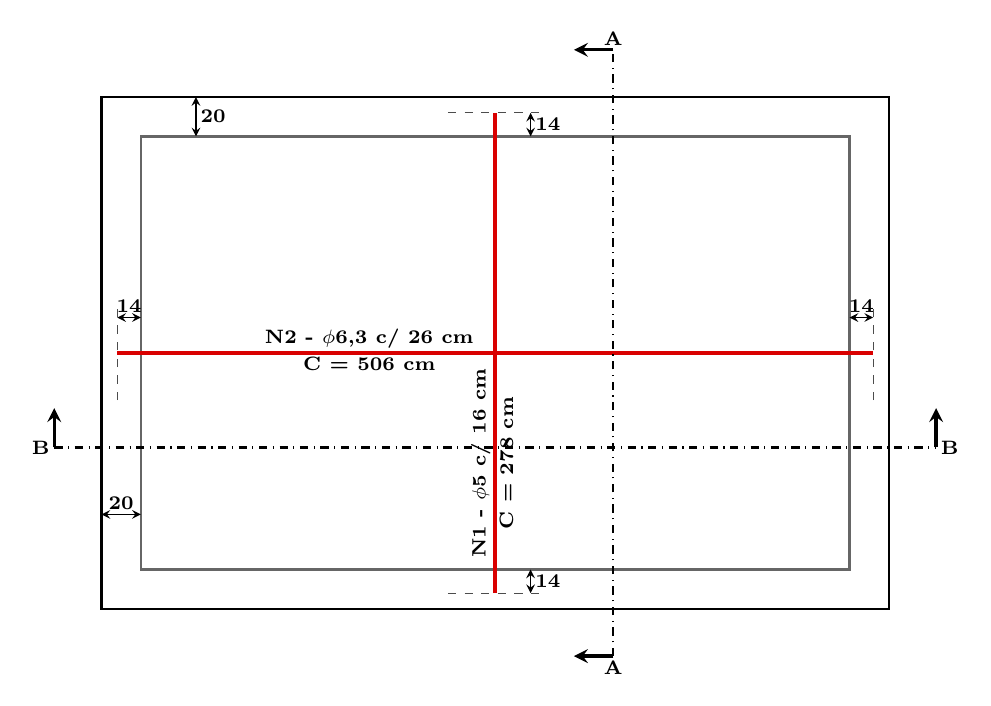
\begin{tikzpicture}[
        scale=1,
        >=stealth,
        contorno/.style={draw=black, thick},
        margem/.style={draw=gray!80!black, thick},
        barra/.style={line width=1.6pt, red!85!black},
        chamada/.style={gray!60!black, thin, dashed},
        cota/.style={<->, thin, black},
        corte/.style={draw=black, dash dot, thick},
        setaCorte/.style={->, very thick, black},
        txt/.style={font=\scriptsize\bfseries, inner sep=1.5pt}
    ]

    % ---------- Parâmetros (planta) ----------
    \def\W{10}      % largura do retângulo maior
    \def\H{6.5}     % altura do retângulo maior (menor que \W)
    \def\m{0.5}     % distância entre os retângulos (= 20 em x e y)
    \def\ext{0.3}   % quanto a barra sai do retângulo menor (< \m)
    \pgfmathsetmacro\cx{\W/2}
    \pgfmathsetmacro\cy{\H/2}
    \pgfmathsetmacro\xa{\cx+1.5}   % posição do corte AA (vertical)
    \pgfmathsetmacro\yb{\cy-1.2}   % posição do corte BB (horizontal)

    % ========== 1. VISTA EM PLANTA ==========
    \draw[contorno] (0,0) rectangle (\W,\H);
    \draw[margem]   (\m,\m) rectangle (\W-\m,\H-\m);

    % Cota da margem (20)
    \draw[cota] (1.2,\H-\m) -- (1.2,\H) node[midway, right, txt] {20};
    \draw[cota] (\m,1.2) -- (0,1.2) node[midway, above, txt] {20};

    % Barra horizontal (principal)
    \draw[barra] (\m-\ext,\cy) -- (\W-\m+\ext,\cy);
    % Barra vertical (secundária)
    \draw[barra] (\cx,\m-\ext) -- (\cx,\H-\m+\ext);

    % Linhas tracejadas nas pontas + cotas em relação ao retângulo menor
    \foreach \xp/\xi in {\m-\ext/\m, \W-\m+\ext/\W-\m} {
        \draw[chamada] (\xp,\cy-0.6) -- (\xp,\cy+0.6);
        \draw[cota] (\xp,\cy+0.45) -- (\xi,\cy+0.45)
            node[midway, above, txt] {14};
    }
    \foreach \yp/\yi in {\m-\ext/\m, \H-\m+\ext/\H-\m} {
        \draw[chamada] (\cx-0.6,\yp) -- (\cx+0.6,\yp);
        \draw[cota] (\cx+0.45,\yp) -- (\cx+0.45,\yi)
            node[midway, right, txt] {14};
    }

    % Valores em cima e em baixo das barras
    \node[txt, above] at (\cx-1.6,\cy) {N2 - $\phi$6,3 c/ 26 cm};
    \node[txt, below] at (\cx-1.6,\cy) {C = 506 cm};
    \node[txt, above, rotate=90] at (\cx,\cy+1.4) {};
    \node[txt, rotate=90, above] at (\cx,\cy-1.4) {N1 - $\phi$5 c/ 16 cm};
    \node[txt, rotate=90, below] at (\cx,\cy-1.4) {C = 278 cm};

    % Cortes AA (vertical) e BB (horizontal)
    \draw[corte] (\xa,-0.6) -- (\xa,\H+0.6);
    \draw[setaCorte] (\xa,\H+0.6) -- ++(-0.5,0);
    \draw[setaCorte] (\xa,-0.6)   -- ++(-0.5,0);
    \node[txt, above] at (\xa,\H+0.6) {A};
    \node[txt, below] at (\xa,-0.6)   {A};

    \draw[corte] (-0.6,\yb) -- (\W+0.6,\yb);
    \draw[setaCorte] (-0.6,\yb)   -- ++(0,0.5);
    \draw[setaCorte] (\W+0.6,\yb) -- ++(0,0.5);
    \node[txt, left]  at (-0.6,\yb)   {B};
    \node[txt, right] at (\W+0.6,\yb) {B};

    %\node[txt] at (\cx,-1.2) {PLANTA DA LAJE};

    \end{tikzpicture}
    %\caption{Planta da laje e cortes AA e BB}
\end{figure}

        \begin{figure}[H]
    \centering
    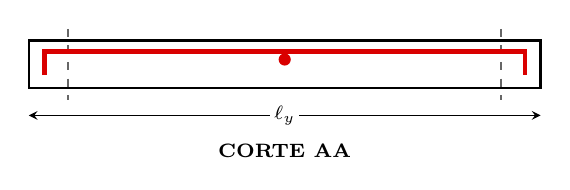
\begin{tikzpicture}[
        scale=1,
        >=stealth,
        contorno/.style={draw=black, thick},
        margem/.style={draw=gray!80!black, thick},
        barra/.style={line width=1.6pt, red!85!black},
        chamada/.style={gray!60!black, thin, dashed},
        cota/.style={<->, thin, black},
        corte/.style={draw=black, dash dot, thick},
        setaCorte/.style={->, very thick, black},
        txt/.style={font=\scriptsize\bfseries, inner sep=1.5pt}
    ]

    % ---------- Parâmetros (planta) ----------
    \def\W{10}      % largura do retângulo maior
    \def\H{6.5}     % altura do retângulo maior (menor que \W)
    \def\m{0.5}     % distância entre os retângulos (= 20 em x e y)
    \def\ext{0.3}   % quanto a barra sai do retângulo menor (< \m)
    \pgfmathsetmacro\cx{\W/2}
    \pgfmathsetmacro\cy{\H/2}
    \pgfmathsetmacro\xa{\cx+1.5}   % posição do corte AA (vertical)
    \pgfmathsetmacro\yb{\cy-1.2}   % posição do corte BB (horizontal)

    %\node[txt] at (\cx,-1.2) {PLANTA DA LAJE};

    % ========== 2. CORTE BB (largura = \W) ==========
    \def\t{0.6}      % espessura da laje no desenho
    \def\dl{0.14}    % posição da armadura (d')
    \def\gh{0.3}     % gancho
    \def\yTop{-3.2}  % topo da laje no corte BB

    % ========== 3. CORTE AA (largura = \H) ==========
    \def\yTopA{-6.4}
    \draw[contorno] (0,\yTopA) rectangle (\H,\yTopA-\t);
    \draw[margem, dashed] (\m,\yTopA+0.15) -- (\m,\yTopA-\t-0.15);
    \draw[margem, dashed] (\H-\m,\yTopA+0.15) -- (\H-\m,\yTopA-\t-0.15);
    % barra secundária (vertical na planta) em comprimento
    \draw[barra] (\m-\ext,\yTopA-\dl-\gh) -- (\m-\ext,\yTopA-\dl)
                 -- (\H-\m+\ext,\yTopA-\dl) -- (\H-\m+\ext,\yTopA-\dl-\gh);
    % barra principal em ponto
    \fill[red!85!black] (\cy,\yTopA-\dl-0.1) circle (2.2pt);
    \draw[cota] (0,\yTopA-\t-0.35) -- (\H,\yTopA-\t-0.35)
        node[midway, fill=white, txt] {$\ell_y$};
    \node[txt] at (\H/2,\yTopA-\t-0.8) {CORTE AA};

    \end{tikzpicture}
    %\caption{Planta da laje e cortes AA e BB}
\end{figure}

        \begin{figure}[H]
    \centering
    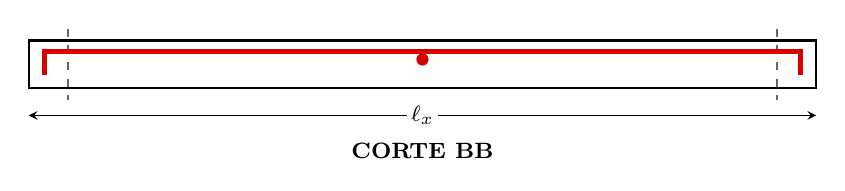
\begin{tikzpicture}[
        scale=1,
        >=stealth,
        contorno/.style={draw=black, thick},
        margem/.style={draw=gray!80!black, thick},
        barra/.style={line width=1.6pt, red!85!black},
        chamada/.style={gray!60!black, thin, dashed},
        cota/.style={<->, thin, black},
        corte/.style={draw=black, dash dot, thick},
        setaCorte/.style={->, very thick, black},
        txt/.style={font=\footnotesize\bfseries, inner sep=1.5pt}
    ]

    % ---------- Parâmetros (planta) ----------
    \def\W{10}      % largura do retângulo maior
    \def\H{6.5}     % altura do retângulo maior (menor que \W)
    \def\m{0.5}     % distância entre os retângulos (= 20 em x e y)
    \def\ext{0.3}   % quanto a barra sai do retângulo menor (< \m)
    \pgfmathsetmacro\cx{\W/2}
    \pgfmathsetmacro\cy{\H/2}

    %\node[txt] at (\cx,-1.2) {PLANTA DA LAJE};

    % ========== 2. CORTE BB (largura = \W) ==========
    \def\t{0.6}      % espessura da laje no desenho
    \def\dl{0.14}    % posição da armadura (d')
    \def\gh{0.3}     % gancho
    \def\yTop{-2.2}  % topo da laje no corte BB

    \draw[contorno] (0,\yTop) rectangle (\W,\yTop-\t);
    \draw[margem, dashed] (\m,\yTop+0.15) -- (\m,\yTop-\t-0.15);
    \draw[margem, dashed] (\W-\m,\yTop+0.15) -- (\W-\m,\yTop-\t-0.15);
    % barra principal em comprimento (ganchos para baixo)
    \draw[barra] (\m-\ext,\yTop-\dl-\gh) -- (\m-\ext,\yTop-\dl)
                 -- (\W-\m+\ext,\yTop-\dl) -- (\W-\m+\ext,\yTop-\dl-\gh);
    % barra secundária em ponto
    \fill[red!85!black] (\cx,\yTop-\dl-0.1) circle (2.2pt);
    \draw[cota] (0,\yTop-\t-0.35) -- (\W,\yTop-\t-0.35)
        node[midway, fill=white, txt] {$\ell_x$};
    \node[txt] at (\cx,\yTop-\t-0.8) {CORTE BB};

    \end{tikzpicture}
    %\caption{Planta da laje e cortes AA e BB}
\end{figure}

        \begin{enumerate}
            \item Comprimento de ancoragem básico \cite[item 9.4.2.4]{nbr6118}
            
            \begin{enumerate}
                \item Resistência da aderência de cálculo \cite[item 9.3.2]{nbr6118}

                $f_{ctk,inf} = 0,7 \ f_{ct,m}$ \cite[item 8.2.5]{nbr6118}

                $f_{ct,m} = 0,3 f_{ck}^{2/3}$ \cite[item 8.2.5]{nbr6118}

                $\gamma_c = 1,4$ \cite[tabela 12.1]{nbr6118} \newline
                
                $f_{ctd} = \frac{f_{ctk, inf}}{\gamma_c} \text{\cite[tabela 8.2]{nbr6118}} \newline f_{ctd} = \frac{0,7 \times 0,3 \times 25^{2/3}}{1,4} =  1,28 \ MPa$ \newline
                
                $\eta_1 = 2,25$ \cite[tabela 8.2]{nbr6118}
                
                $\eta_2 = 1$ \cite[item 9.3.1]{nbr6118}
                
                $\eta_3 = 1$ \cite[item 9.3.2.1]{nbr6118} \newline
                
                $f_{bd} = \eta_1 \ \eta_2 \ \eta_3 f_{ctd} = 2,25 \times 1 \times 1 \times 1,28 = 2,89 \ MPa$ \newline
            \end{enumerate}

            $\gamma_s = 1,15$ \cite[tabela 12.1]{nbr6118}

            $f_{yd}=\frac{f_{yk}}{\gamma_s}$ \newline

            $\ell_b = \frac{\phi}{4}\frac{f_{yd}}{f_{bd}} \geq 25 \phi \newline \ell_b = \frac{\times 0,5}{4}\frac{\frac{500}{1,15}}{2,89} \geq 25 \times 0,5 \newline \ell_b = 18,81  \geq 12,5$ \newline

            \item Comprimento de ancoragem necessário \cite[item 9.4.2.5]{nbr6118}
            
            \begin{observacao}
                $1$ para ficar a favor da segurança.
            \end{observacao}

            $\alpha = 1$ \cite[item 9.4.2.5]{nbr6118} \newline

            $\ell_{b,nec} = \alpha\ \ell_b \frac{A_{s,calc}}{A_{s,ef}} \geq  \ell_{b,min} \newline \ell_{b,nec} = \alpha\ \ell_b \cancelto{1}{\frac{A_{s,calc}}{A_{s,ef}}} \geq \begin{cases}
                0,3 \ell_b = 0,3 \times 18,81 = 5,64 \ cm \\
                10\phi = 10 \times 0,5 = 5 \ cm \\
                10 \ cm
            \end{cases} \newline \ell_{b,nec} = 1 \times 18,81 = 18,81 \geq 10 \ cm$
        \end{enumerate}
        
        \fbox{L2}
        
        \fbox{L3}
        
        \fbox{L4}
        
    \end{enumerate}
\end{resposta}